\documentclass{article}
\usepackage[utf8]{inputenc}

\title{ UBusy Design }
\author{ Kitteh Rong }
\date{June 2011}

\usepackage{natbib}
\usepackage{graphicx}

\begin{document}

\maketitle

\tableofcontents

\abstract{This is a design document about the Ubusy Android app. It contains information about customers, usability data, requirements gathering, use case analysis and other demographics for determining and appropriate design.}

\section{Description}
 %% Type in something about the app

\section{Use Cases}

\begin{figure}[h!]
\centering
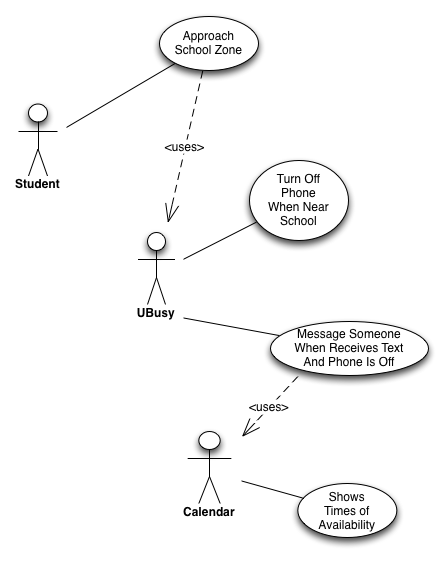
\includegraphics[scale=1.7]{Diagrams/UseCases1.png}
\caption{Use Cases for the UBusy App}
\label{threadsVsSync}
\end{figure}

\subsection{Functional Requirements}


\subsection{Usability Requirements}

\subsection{Flow}


%\begin{figure}[h!]
%\centering
%\includegraphics[scale=1.7]{universe.jpg}
%\caption{The Universe}
%\label{threadsVsSync}
%\end{figure}

\section{Conclusion}
%``I always thought something was fundamentally wrong with the %universe'' \citep{adams1995hitchhiker}

\bibliographystyle{plain}
\bibliography{references}
\end{document}
